\section{What has been tested against what}
\label{sec:coverage}

\subsection{Building the matrix}

We cross-reference the mechanism census against the defense census and record a
pair only when a paper \emph{evaluated} the defense against that named
mechanism. A claim that a defense addresses a problem is not a pair. We mined
each defense paper's baselines, results and technical description for named
mechanisms actually tested against, and favoured false negatives over false
positives.

Reading only defense papers biases the matrix, because a defense paper chooses
which attacks to run. We therefore added a reverse pass over the \emph{attack}
papers, which report a defense losing in a way no defense paper will. The
reverse scan covered the full mechanism registry and recovered 54 pairs that
the defense-side scan had missed, 12 of them against mechanisms that had no
tested defense at all. The final matrix holds \textbf{\NPairsComposite{}
confirmed pairs}.\footnote{Three denominators appear in this paper and we keep them
distinct. 332 is the full matrix, including the supplementary passes and the
reverse scan. 233 is the base matrix from defense-paper reads alone. 232 is the
subset for which we could also determine the reporting side and the reported
outcome, which is the base used in Section~\ref{sec:whoran} and for the
same-track rate in Section~\ref{sec:literatures}. All three are produced by
one script from the registries, and \NPairsComposite{} supersedes the 332
published in RQ5, which predates reverse-scan pass 3.}

\subsection{The matrix is sparse, and sparse in a specific way}

\begin{itemize}
\item \textbf{\NDefMatchedFull{} of \NDefenses{} defenses
  (\PctDefMatched{}\%)} have at least one confirmed test against a named
  mechanism. The rest were not evaluated against anything our registry
  recognizes as a distinct named technique. \emph{That is not the same as
  untested}, and the distinction matters enough that we audited it
  separately: see below.
\item \textbf{\NMechUncovered{} of \NMechanismsBench{} mechanisms
  (\PctMechUncovered{}\%) have zero defenses} evaluated against them.
\item \textbf{\NDefMatchedFull{} defenses appear in at least one pair, and
  \NDefOneFull{} of them (\PctDefOneFull{}\%) appear in exactly one.}
  Thirty-four appear in two, 23 in three, and \NDefFourPlus{} in four or
  more. The most cross-tested defense appears in \NDefCeiling{} pairs.
\end{itemize}

The third point needs care, because the answer depends on which evidence you
count, and the difference is itself a finding.

\textbf{Counting only what defense papers report, there is essentially no
generalist defense.} In the base matrix, built from defense-paper reads alone,
\NDefOneBase{} of \NDefMatchedBase{} matched defenses (\PctDefOneBase{}\%)
were tested against exactly one mechanism,
and cross-mechanism testing tops out at three mechanisms, twice, in a corpus
of \NCorpus{} papers.

\textbf{Adding the attack-paper scan raises the ceiling, but changes what
breadth means.} On the full pair set the most-tested defense appears against
\NDefCeiling{} distinct named attacks, and \NDefFourPlus{} defenses appear
against four or more. Of the pairs belonging to those \NDefFourPlus{}, 46\% were contributed by attack papers rather
than by the defenses' own evaluations. For the single broadest case, SecAlign,
seven of its eight pairs come from attack papers. Its breadth is not evidence
that it was evaluated widely by its authors. It is evidence that attackers
chose it as a target, and by Table~\ref{tab:whoran} those are pairs the defense
lost.

So the two readings do not conflict. Defense authors test narrowly. The
defenses that look broadly tested are mostly the ones that attracted attackers.
Either way, a claim that a method provides broad protection against context
poisoning is, on the current evidence, untested rather than wrong.

\subsection{How much of the gap is the field, and how much is us}

A coverage matrix measures resolution against a named registry. It is easy to
read the complement as "never tested", and that reading is wrong. A defense
paper that runs on AgentDojo without naming which injection it used is
evaluated adversarially. It is not a (defense, mechanism) pair, because
expanding a benchmark to all of its constituent attacks would manufacture
coverage, and we refuse that expansion throughout. It is not untested either.

We therefore audited the \NDefenses{} defenses against a coarser question: did
anyone run any comparison at all? \textbf{14 defenses (2.7\%) report no
baseline comparison of any kind.} Each of the 14 was confirmed by hand. Their
own evaluation sections say so: "No comparison against existing forensic or
IPI-detection methods is reported", "No empirical baselines. The comparison is
conceptual", "authors explicitly acknowledge the absence of a baseline method
comparison". One proposes a defense with no implementation at all.

So the honest statement of the gap is narrower than the matrix alone suggests.
\textbf{Most defenses were evaluated. What most of them were not evaluated
against is a second named mechanism, and what almost none were evaluated
against is the other community's threat model} (Section~\ref{sec:literatures}).
A keyword audit of the remaining evaluation descriptions is reported in the
artifact, but we do not quote its middle categories here: hand-checking showed
roughly half of its flagged cases were classifier misses rather than real
ones, which is the same claim-versus-evidence error this paper is about and is
not a basis for a number in a systematization.

\subsection{The result depends on who ran the experiment}
\label{sec:whoran}

The reverse scan makes a second measurement possible. For every pair we also
record which side of the field reported it, and what outcome was reported.

\begin{figure}[t]
\centering
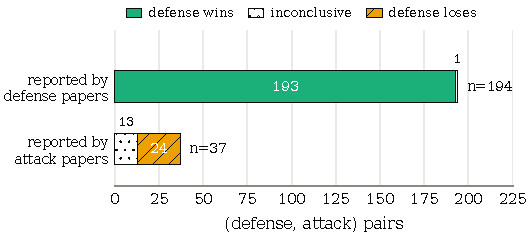
\includegraphics[width=\columnwidth]{figures/fig3_who_reports}
\caption{The same defenses and the same attacks, reported by the two sides of
the field. A defense paper reports its defense winning in 193 of 194 pairs. An
attack paper reports the defense winning in none of 37.}
\label{fig:whoreports}
\end{figure}

\begin{table}[t]
\caption{Reported outcome of a (defense, attack) pair, by who reported it.
Same defenses. Same attacks. Opposite verdicts.}
\label{tab:whoran}
\small
\begin{tabular}{@{}lrrr@{}}
\toprule
\textbf{Reported by} & \textbf{Pairs} & \textbf{Defense wins} &
\textbf{Defense loses} \\
\midrule
defense papers & 194 & \textbf{193} & 0 \\
attack papers  &  37 & \textbf{0}   & 24 \\
\bottomrule
\end{tabular}
\end{table}

\textbf{When a defense paper reports a pair, the defense wins 193 times out of
194. When an attack paper reports a pair, the defense wins zero times out of
37.} The remaining attack-paper pairs are inconclusive rather than wins.

We are not claiming misconduct. Each side runs the experiment it has reason to
run, under conditions it chose, and publishes what it finds. An attack paper
exists because its attack works, so it selects defenses its attack defeats. A
defense paper exists because its defense works, so it selects attacks its
defense stops. Both selections are rational and both are published in good
faith.

The consequence is still that \textbf{the published outcome of a
(defense, attack) pair is close to fully determined by which side wrote the
paper}, and the two sides rarely write about the same pairs. A reader
assembling a picture of "what works" from defense papers alone, which is what
the citation data in Section~\ref{sec:literatures} suggests most readers do,
will assemble one in which defenses essentially always work.

This is the strongest argument we can make for the experiments that follow.
When a literature's reported outcomes are this strongly conditioned on
authorship, the only way to learn what a defense does against an attack it was
not built for is to run it.
